\documentclass[12pt, letterpaper]{article}

% --- FONTS: HELVETICA ---
\usepackage[scaled]{helvet}
\renewcommand{\familydefault}{\sfdefault}
\usepackage[T1]{fontenc}
\usepackage[utf8]{inputenc}

% --- FIX MATH SYMBOLS ---
\usepackage[helvet]{sfmath}
\DeclareMathAlphabet{\mathcal}{OMS}{cmsy}{m}{n}


% --- PACKAGES ---
\usepackage[margin=1in]{geometry}
\usepackage{amsmath, amssymb, amsfonts}
\usepackage{graphicx}
\usepackage{algorithm}
\usepackage{algorithmic}
\usepackage{booktabs}
\usepackage{url}
\usepackage{cite} 
\usepackage[colorlinks=true, linkcolor=blue, citecolor=blue, urlcolor=blue]{hyperref}
\usepackage{titlesec}
\usepackage{authblk}
\usepackage{float}
\usepackage{subcaption}
\graphicspath{{figs/}} 
\usepackage[section]{placeins}

\usepackage{url}  % Formatting web addresses
\usepackage{ifthen}  % Conditional
\usepackage{multicol}   %Columns
\usepackage[utf8]{inputenc} %unicode support
\usepackage{amsmath}
\usepackage{amssymb}
\usepackage{epsfig}
\usepackage{epstopdf}
\usepackage{graphicx}
\usepackage[margin=0.1pt,font=footnotesize,labelfont=bf]{caption}
\usepackage{setspace}
%\usepackage{longtable}
\usepackage{colortbl}
%\usepackage{palatino,lettrine}
%\usepackage{times}
%\usepackage[applemac]{inputenc} %applemac support if unicode package fails
%\usepackage[latin1]{inputenc} %UNIX support if unicode package fails
\usepackage[wide]{sidecap}
%\usepackage[authoryear,round,comma,sort&compress]{natbib}
\usepackage[square,sort,comma,numbers,sort&compress]{natbib}
%\usepackage[authoryear,round]{natbib}
\usepackage{simplemargins}
\usepackage{fullpage}
\usepackage{comment}
\usepackage{textcomp}
\usepackage{amsmath}
%\usepackage[space]{cite}
\urlstyle{rm}

\usepackage{lineno}
\usepackage{supertabular}
\usepackage{multirow}
\usepackage{booktabs}
\usepackage{longtable}
\usepackage{lscape}

% --- CUSTOM OPERATORS ---
\def\R{\mathbb{R}}
\def\Eps{\mathcal{E}}
\def\E{\mathbb{E}}
\def\Z{\mathbb{Z}}
\def\V{\mathbb{V}}
\def\F{\mathcal{F}}
\def\G{\mathcal{G}}
\def\H{\mathcal{H}}
\def\S{\mathcal{S}}
\def\D{\mathcal{D}}
\def\P{\mathbb{P}}
\def\1{\mathbf{1}}
\def\n{\nappa}
\def\h{\mathbf{w}}
\def\v{\mathbf{v}}
\def\x{\mathbf{x}}
\def\X{\mathcal{X}}
\def\Y{\mathcal{Y}}
\def\eps{\epsilon}
\def\y{\mathbf{y}}
\def\e{\mathbf{e}}
\DeclareMathOperator*{\argmin}{arg\,min}
\DeclareMathOperator*{\argmax}{arg\,max}
\setlength\bibsep{0pt}
\renewcommand{\rmdefault}{phv}\renewcommand{\sfdefault}{phv}
\newcommand{\norm}[1]{\left\lVert#1\right\rVert}

% Change the number format in the ref list -
\renewcommand{\bibnumfmt}[1]{#1.}

% Change Figure to Fig.
\renewcommand{\figurename}{Fig.}

% --- HEADING STYLES ---
% \titleformat{\section}{\normalfont\Large\bfseries}{\thesection}{1em}{}
% \titleformat{\subsection}{\normalfont\large\bfseries}{\thesubsection}{1em}{}
% \titleformat{\subsubsection}{\normalfont\normalsize\bfseries}{\thesubsubsection}{1em}{}

\makeatletter
\renewcommand\subsection{\@startsection
	{subsection}{2}{0mm}
	{-0.05in}
	{-0.5\baselineskip}
	{\normalfont\normalsize\bfseries}}
\renewcommand\subsubsection{\@startsection
	{subsubsection}{2}{0mm}
	{-0.05in}
	{-0.5\baselineskip}
	{\normalfont\normalsize\itshape}}
\renewcommand\section{\@startsection
	{subsection}{2}{0mm}
	{-0.2in}
	{0.05\baselineskip}
	{\normalfont\large\bfseries}}
\renewcommand\paragraph{\@startsection
	{paragraph}{2}{0mm}
	{-0.05in}
	{-0.5\baselineskip}
	{\normalfont\normalsize\itshape}}
\makeatother

\doublespace

% --- METADATA ---
\title{\textbf{Hybrid Hidden Markov Model for Modeling Equity Return Dynamics: A Discrete-State Approach with Jump-Diffusion}}
\author{Abdulrahman Alswaidan}
\author{Jeffrey Varner\,$^{*}$}
\affil{Smith School of Chemical and Biomolecular Engineering, College of Engineering, Cornell University, Ithaca, NY 14850}
% \date{\today}


\begin{document}
\maketitle

\begin{abstract}
\noindent Financial time series exhibit persistent statistical regularities, commonly referred to as stylized facts, that are not captured by classical Gaussian diffusion models. In particular, empirical equity returns display heavy-tailed distributions, negligible linear autocorrelation, and pronounced volatility clustering. This work proposes a hybrid hidden Markov modeling framework that discretizes continuous excess growth rates into quantile-defined market states and augments the resulting regime-switching process with a Poisson-driven jump-diffusion mechanism. Model parameters are estimated empirically through transition counting, avoiding the computational complexity of likelihood maximization and expectation-maximization procedures. A modular pipeline was developed to support the construction of return models for any ticker; we validated the framework using SPY as a representative asset, though the framework is applicable to any ticker within our 424 asset dataset. Using more than 2,500 trading days of data, we demonstrate that while standard regime-switching models can reproduce marginal return distributions, the inclusion of a jump-duration mechanism is essential for generating persistent extreme-volatility regimes. The selection of $N=90$ states provides an adequate balance between distributional fidelity and statistical robustness, successfully reproducing heavy-tailed behavior and volatility clustering in both in-sample and out-of-sample settings.
\end{abstract}

\vspace{0.5cm}
{\par \centering $^{*}$Corresponding author:}
{\par \centering Jeffrey D. Varner,}
{\par \centering Professor, School of Chemical and Biomolecular Engineering,}
{\par \centering 256A Olin Hall, Cornell University, Ithaca NY, 14853}
{\par \centering Email: jdv27@cornell.edu}
{\par \centering Phone: (607) 255 - 4258}
{\par \centering Fax: (607) 255 - 9166}

\newpage

\section*{Introduction}
The quantitative modeling of financial markets has long faced the challenge of reconciling the theoretical implications of the efficient markets hypothesis (EMH) with the empirical complexity of observed price dynamics. Under the EMH, asset prices fully reflect all available information, implying that price changes follow a martingale process with no exploitable predictability \cite{fama_efficient_1970}. This perspective motivated the widespread adoption of geometric Brownian motion (GBM) as a canonical model for asset prices, yet decades of data show systematic departures from Gaussian assumptions, including heavy-tailed return distributions, volatility clustering, and intermittent extreme events \cite{mandelbrot_variation_1963, cont_empirical_2001}. These stylized facts are robust across asset classes and time periods, and they matter practically because they govern tail risk, drawdown behavior, and the persistence of stress regimes that dominate portfolio outcomes.

This study focuses on three core properties: leptokurtic return distributions, the absence of linear autocorrelation in raw returns, and the persistence of volatility. The first two properties motivate models that can preserve marginal distributional shape without introducing spurious predictability, while the third points to slow-moving higher-order dependence that is not captured by diffusion alone. A range of alternative approaches address these issues from different angles: ARCH/GARCH-family models target conditional variance dynamics \cite{engle_1982, bollerslev_garch_1986}; stochastic-volatility and jump-diffusion models introduce latent variance or discontinuities to enrich tails \cite{heston_stochastic_1993, merton_jump_1976}; and data-driven sequence models, including recurrent neural networks and LSTM variants, have been used for return and volatility prediction and, in probabilistic form, can emit full predictive distributions \cite{elman_rnn_1990, hochreiter_lstm_1997, fischer_krauss_2018, salinas_deepar_2020, liu_rnn_volatility_2017, choi_arima_lstm_2018, alparslan_gamestop_2021}. While useful, these approaches either emphasize conditional variance over regime duration, require intensive likelihood-based estimation, or sacrifice interpretability and explicit control over regime persistence. Hidden Markov models (HMMs) and related regime-switching frameworks offer a probabilistic structure for non-stationary market behavior through latent state dynamics \cite{rabiner_introduction_1986}, yet standard HMM specifications often fail to generate persistent high-volatility regimes, leading to overly rapid reversion following extreme events \cite{ryden_stylized_1998, bulla_stylized_2006}. Bridging this gap requires a model that preserves distributional fidelity while also enforcing realistic duration in extreme regimes.

We address this challenge by developing a hybrid HMM framework that discretizes continuous excess growth rates into quantile-based regimes and augments the resulting Markov process with a jump-duration mechanism that enforces volatility persistence, linking smooth diffusion to discontinuous shocks identified by jump-detection methods \cite{au_yeung_jump_2020}. Using a 424-asset dataset and SPY as a representative case study, we estimate transition dynamics empirically and validate the model through in-sample and out-of-sample tests on distributional fit and volatility clustering. We find that a state resolution of $N=90$ provides a practical balance between fidelity and statistical robustness, and that the jump-duration extension is essential for reproducing persistent extreme-volatility regimes that standard regime-switching models miss. Future work will extend the framework to multi-asset portfolios, alternative state encodings, and higher-frequency data where jump identification and regime persistence play an even larger role in stress testing and scenario design.

\section*{Materials and Methods}\label{sec:methods}

\subsection*{Dataset and modular pipeline}
The empirical foundation of this study is a comprehensive dataset composed of 424 U.S.-listed equities and exchange-traded funds spanning 2,515 trading days. A modular pipeline was developed to support the automated construction of return models for any ticker within this dataset, allowing for high-throughput simulation and stress testing across diverse market sectors. To validate the performance of this pipeline, we focused our analysis on the representative single-asset SPY, which tracks the S\&P 500 index. The data includes daily open, high, low, and close prices along with volume-weighted average price metrics (VWAP). For training purposes, the first 2,515 observations constitute the in-sample dataset, spanning from January 3, 2014, to December 29, 2023. A subsequent 277 trading days, from January 2, 2024, to February 7, 2025, are reserved for out-of-sample testing to assess model generalizability. This daily resolution allows the framework to identify the long-term statistical regularities and stylized facts suggested by market microstructure theory.

\subsection*{Excess growth rate calculation}
We compute the excess growth rate $R_{i,j}$ for a given equity price series $P_{i,j}$ using VWAP data. In this formulation, the index $i$ represents a specific equity within the dataset, while the index $j$ denotes the discrete time step. To isolate the stochastic premium earned over a risk-free asset, the excess growth rate is defined as:
\begin{equation}
    R_{i,j} \equiv \left( \frac{1}{\Delta t} \right) \cdot \ln \left( \frac{P_{i,j}}{P_{i,j-1}} \right) - r_f
    \label{eq:growth_rate}
\end{equation}
In this expression, $\Delta t$ represents the time step set to $1/252$ for daily data. Log returns are utilized because they are time-additive, allowing for the consistent aggregation of returns over long horizons. To ensure the model aligns with modern capital asset pricing theory, we subtract a constant risk-free rate $r_f = 0.0421$; this value represents the 10-year Treasury yield observed on June 17, 2024. While $r_f$ varies dynamically over the sample period, a constant proxy is employed here to isolate the endogenous volatility dynamics without introducing exogenous rate-curve noise.

\subsection*{Discrete hidden Markov model encoding via quantile binning}
We define the hidden Markov model using the tuple $\mathcal{M} = (\mathcal{S}, \mathcal{O}, \mathbf{T}, \mathbf{E}, \bar{\pi})$ \cite{rabiner_introduction_1986}. To construct an observable Markov model, we transform the continuous return series into a symbolic sequence of market regimes by partitioning the cumulative distribution function (CDF) of the returns into $N$ states. In this framework, we utilize the Laplace distribution as a parametric model to fit the empirical returns and define the state partitions.

The choice of the Laplace distribution over alternatives such as the Student's t-distribution is motivated by its structural alignment with the sharp peaks and heavy tails characteristic of high-frequency financial returns \cite{cont_empirical_2001, kotz_laplace_2001}. While the Student's t-distribution is frequently used to model leptokurtosis, the Laplace distribution's cusp-like peak at the mean more accurately characterizes the high concentration of small price movements observed in the SPY dataset \cite{mandelbrot_variation_1963, harwood_against_2019}. Furthermore, the Laplace distribution provides a computationally efficient closed-form for quantile estimation, facilitating the high-throughput needs of the modular 424-ticker pipeline. While maximum likelihood estimation for the Student's t-distribution often requires iterative numerical overhead, the Laplace distribution allows for a direct MLE approach \cite{bilmes_gentle_nodate}. Choosing a quantile-based approach based on this parametric fit ensures that each state is informed by an equal number of historical observations, providing significant statistical stability and alignment with value-at-risk models \cite{manganelli_2004}. By utilizing the Laplace distribution to inform the binning process, the model gains a structured baseline for characterizing the peak and tails of the return series before the empirical transition logic and jump-diffusion mechanism are applied \cite{kou_jump-diffusion_2002}.

\subsection*{Empirical parameter estimation}
We estimate the transition matrix $\mathbf{T}$ through direct frequentist counting rather than iterative optimization. This approach differs from the traditional expectation-maximization (EM) algorithm used for parameter estimation in Gaussian mixture and hidden Markov models \cite{bilmes_gentle_nodate}. The stationary distribution $\bar{\pi}$ represents the long-run probability of the market occupying various regimes or moods \cite{hamilton_regime_2018}. While $\bar{\pi}$ mathematically satisfies the balance equation $\bar{\pi} = \bar{\pi}\mathbf{T}$, we estimate this distribution numerically by raising the transition matrix $\mathbf{T}^n$ to a sufficiently large power $n = 50$, ensuring the vector reflects the global equilibrium of market dynamics \cite{grinstead_introduction_1997}.

\subsection*{Hybrid jump-diffusion extension}
Empirical transition matrices often have low probabilities for exiting central states into extreme tail-states, causing models to lose the effect of volatility clustering too quickly \cite{bulla_stylized_2006}. We correct this by adding jump parameters $\epsilon$, representing the probability of a jump event, and $\lambda$, representing the mean duration. If a jump is triggered, the jump-duration $K$ is sampled from a Poisson distribution such that $K \sim \text{Poisson}(\lambda)$, which is standard for modeling independent events in fixed intervals \cite{glasserman_monte_2003}. During these $K$ steps, the standard Markovian transitions are overridden to target tail-states.

\subsection*{State decoding and reconstruction}
To characterize the returns within each regime, we fit local normal distributions $\mathcal{N}(\mu_k, \sigma_k)$ to each individual quantile-bin using maximum-likelihood estimation. During simulation, when the model is in state $k$, the continuous decoded growth rate ($\hat{R}_t$) is sampled from the corresponding local distribution. This hybrid approach ensures that the model preserves the discontinuous components of the price process essential for realistic asset modeling while maintaining a smooth representation of intra-state variance \cite{kou_jump-diffusion_2002}.

\section*{Results and Discussion}
We simulated 1,000 paths of 2,515 trading days using VWAP price data for both the standard model with no-jumps and the hybrid model with jumps. The optimal jump parameters $\epsilon$ and $\lambda$ were identified through a multi-objective grid search designed to minimize the combined error between simulated and observed market signatures. Specifically, the search targeted the autocorrelation function (ACF) of absolute growth rates to capture volatility clustering and the global kurtosis to ensure heavy-tailed fidelity. The grid explored $\epsilon$ values from $0.00001$ to $0.0001$ and $\lambda$ values from $1.0$ to $100.0$. The error function utilized a kurtosis penalty weight of $0.20$ to prioritize tail behavior alongside the squared error of the ACF lags.

Optimized jump parameters ($\epsilon \approx 5 \times 10^{-5}$ and $\lambda \approx 67$) reproduced the heavy-tailed kurtosis and ARCH effect observed in SPY (Figure \ref{fig:wj_90_combo}). Based on the statistical consistency results, the configuration with $N=90$ states was deemed an adequate resolution and is used for synthetic data generation and analysis in this study. Increasing the number of states $N$ enhances the granularity of the market regimes, leading to a more precise fit for in-sample results. While it becomes trivial to add more states, there is a practical limit to this refinement; if $N$ is excessively large, such as 350 states, the empirical estimation protocol fails because the historical dataset becomes too sparse relative to the state space. In such cases, certain states may never be visited, resulting in zero transition probabilities that break the mathematical integrity of the Markov chain. Conversely, a very small number of states, such as $N=10$, results in a coarse-grained model that misses the critical heavy tails observed in the empirical data. Therefore, the selection of $N=90$ provides a sufficient balance between distributional fidelity and statistical robustness. The analysis is divided into in-sample evaluations, spanning from January 3, 2014, to December 29, 2023, totaling 2,515 trading days, and out-of-sample testing, which covers 277 trading days from January 2, 2024, to February 7, 2025.

In-sample KS and AD tests showed pass rates above 98\% for both model variants (Table \ref{tab:statistical_results}), indicating strong distributional alignment across 2,515 trading days. We performed Kolmogorov-Smirnov and Anderson-Darling tests for each case using a $p$-value cutoff of 0.05.

\begin{table}[htpb]
\centering
\caption{Statistical consistency of simulated growth rates across hidden Markov model configurations.}
\label{tab:statistical_results}
\begin{tabular}{@{}lccc@{}}
\toprule
\textbf{model type} & \textbf{number of states ($N$)} & \textbf{KS test pass rate} & \textbf{AD test pass rate} \\ \midrule
standard (no-jumps) & 90 & 99.4\% & 98.4\% \\
hybrid (with jumps) & 90 & 99.5\% & 98.1\% \\ \bottomrule
\end{tabular}
\end{table}

The standard no-jumps model matched the marginal distribution but failed to capture volatility clustering (Figure \ref{fig:nj_90_combo}). The autocorrelation of absolute growth in subplot (c) remains flat, showing that state resolution alone cannot overcome the memoryless limitations of standard transition logic.

\begin{figure}[htpb]
    \centering
    \begin{subfigure}[b]{0.48\textwidth}
        \centering
        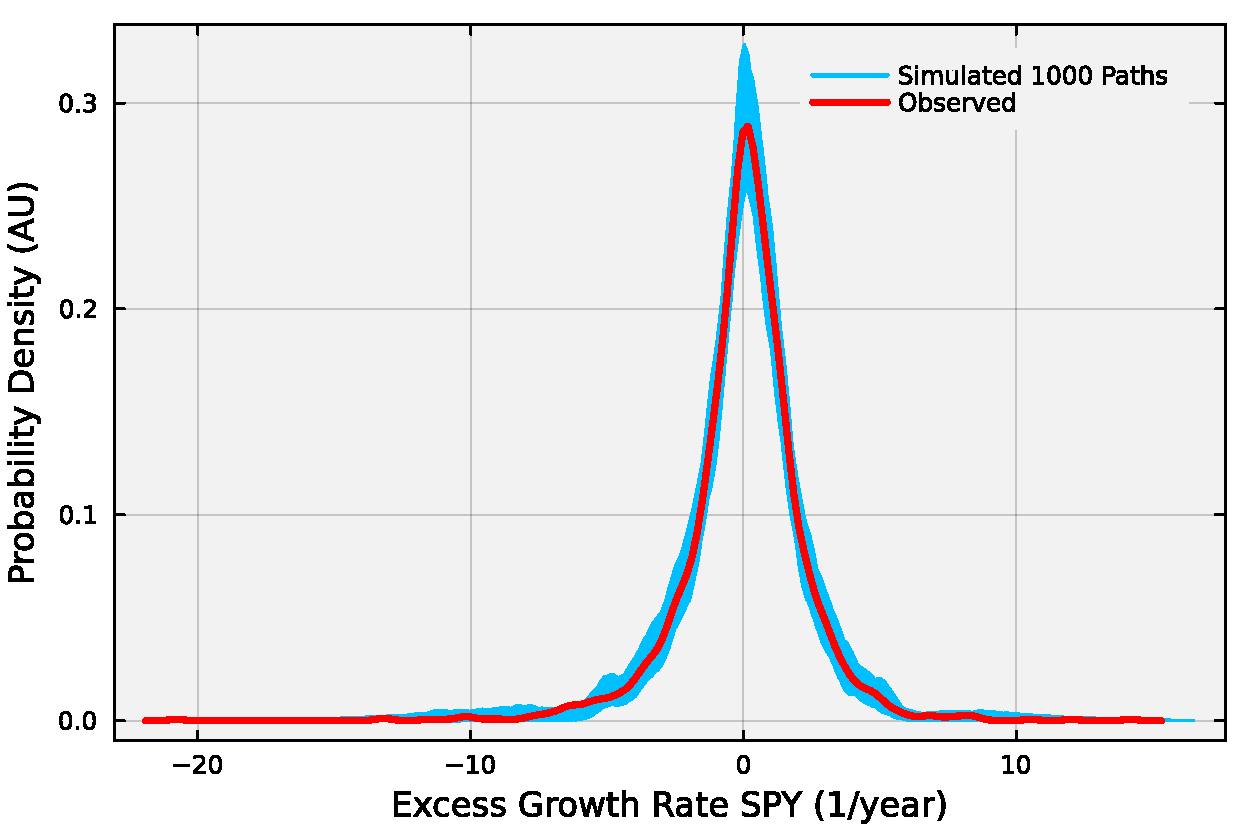
\includegraphics[width=\textwidth]{Fig-SPY-90-InSample-Density-Comparison-NJ.pdf}
        \caption{Probability density comparison}
    \end{subfigure}
    \hfill
    \begin{subfigure}[b]{0.48\textwidth}
        \centering
        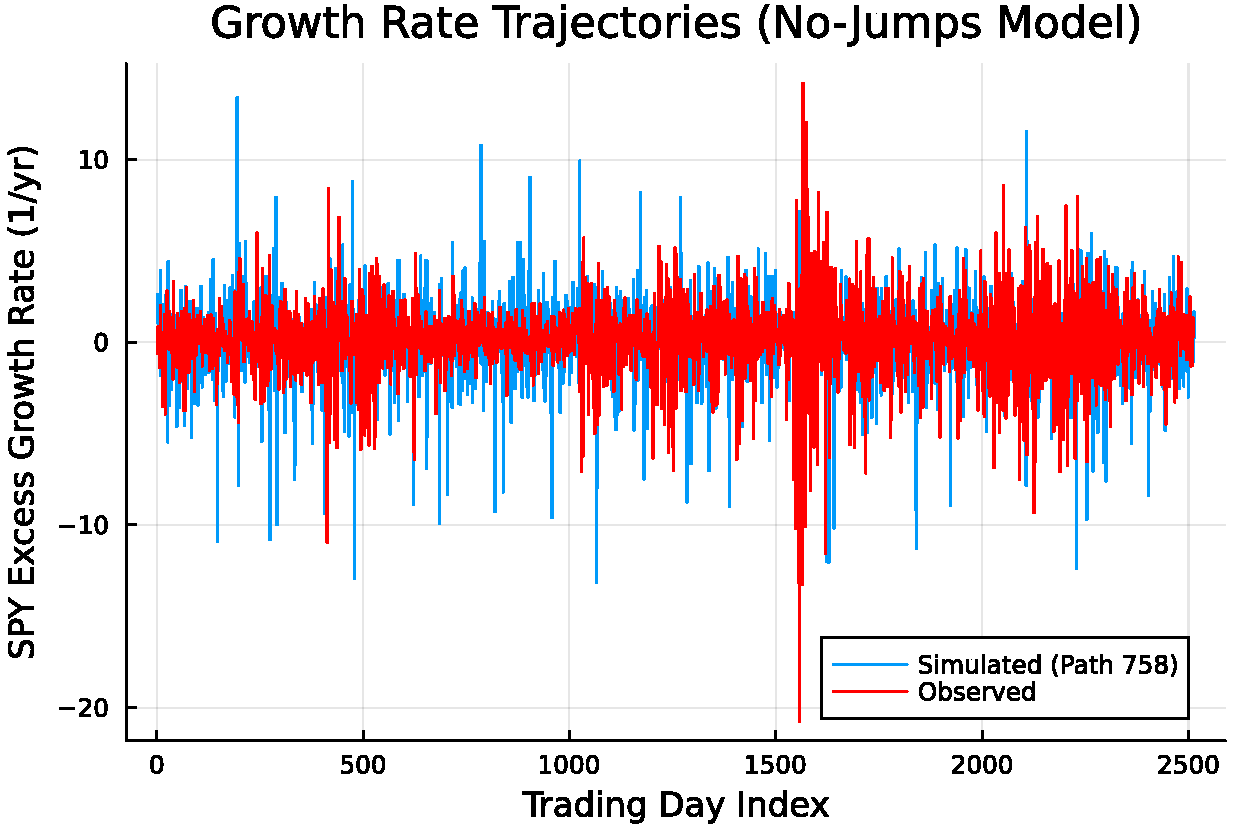
\includegraphics[width=\textwidth]{Fig-SPY-90-InSample-Return-Trajectories-NJ.pdf}
        \caption{Growth rate trajectories}
    \end{subfigure}
    \vspace{0.3cm}
    \begin{subfigure}[b]{0.48\textwidth}
        \centering
        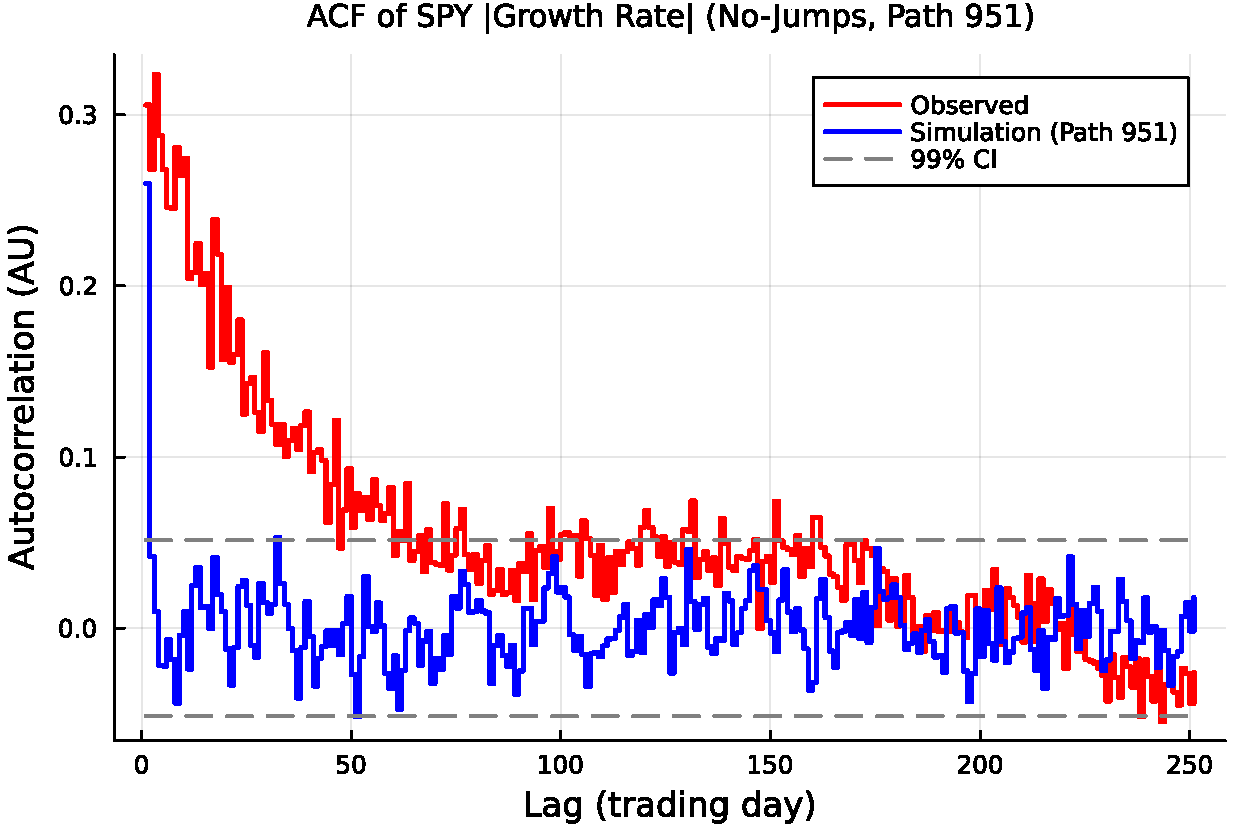
\includegraphics[width=\textwidth]{Fig-SPY-90-ACF-Absolute-Growth-NJ.pdf}
        \caption{Absolute growth autocorrelation}
    \end{subfigure}
    \hfill
    \begin{subfigure}[b]{0.48\textwidth}
        \centering
        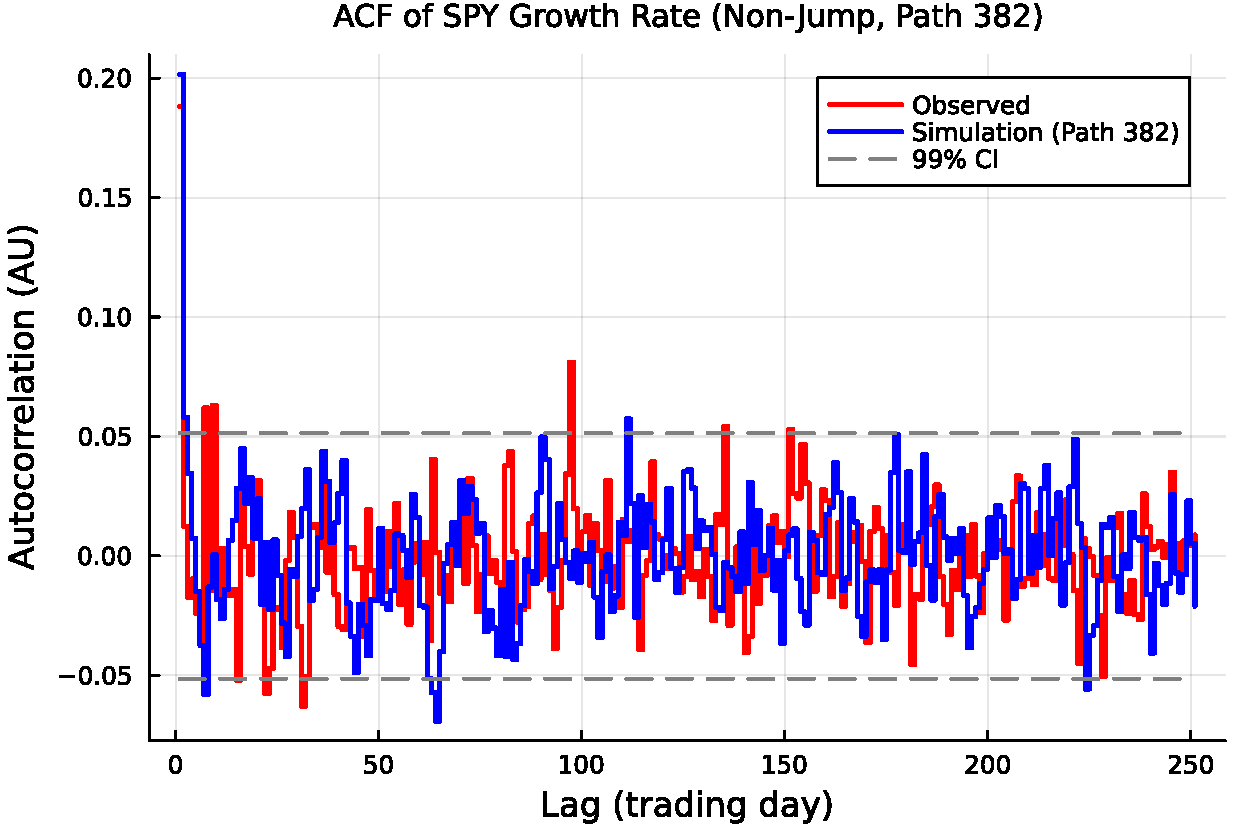
\includegraphics[width=\textwidth]{Fig-SPY-90-ACF-Growth-NJ.pdf}
        \caption{Growth autocorrelation function}
    \end{subfigure}
    \caption{Performance of the standard no-jumps model using $N=90$ states.}
    \label{fig:nj_90_combo}
\end{figure}

The hybrid model reproduced volatility clustering, with the absolute-growth autocorrelation mirroring the ARCH effect (Figure \ref{fig:wj_90_combo}). With $N=90$ states, this configuration provides a practical balance and aligns with advanced volatility estimation techniques using HMM architectures \cite{rossi_volatility_2006}.

\begin{figure}[htpb]
    \centering
    \begin{subfigure}[b]{0.48\textwidth}
        \centering
        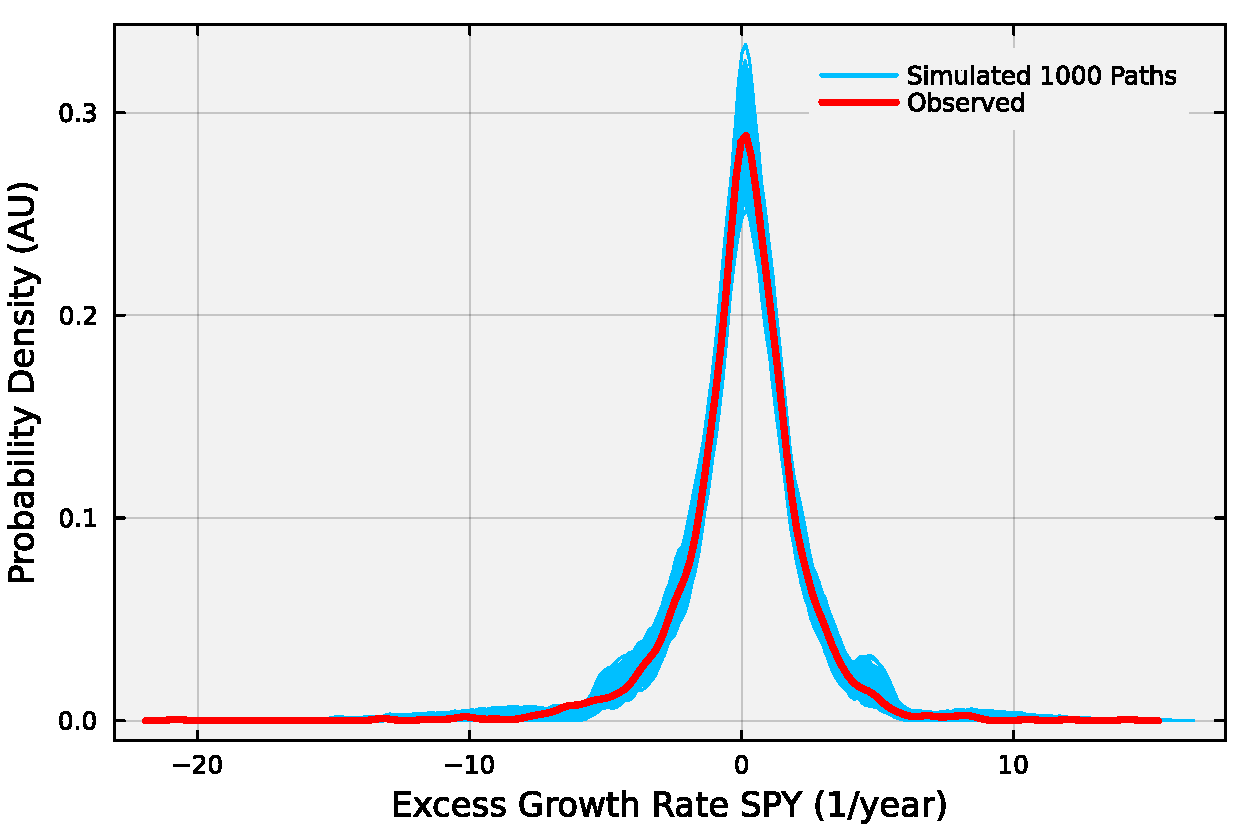
\includegraphics[width=\textwidth]{Fig-SPY-90-InSample-Density-Comparison-HMM-WJ.pdf}
        \caption{Probability density comparison}
    \end{subfigure}
    \hfill
    \begin{subfigure}[b]{0.48\textwidth}
        \centering
        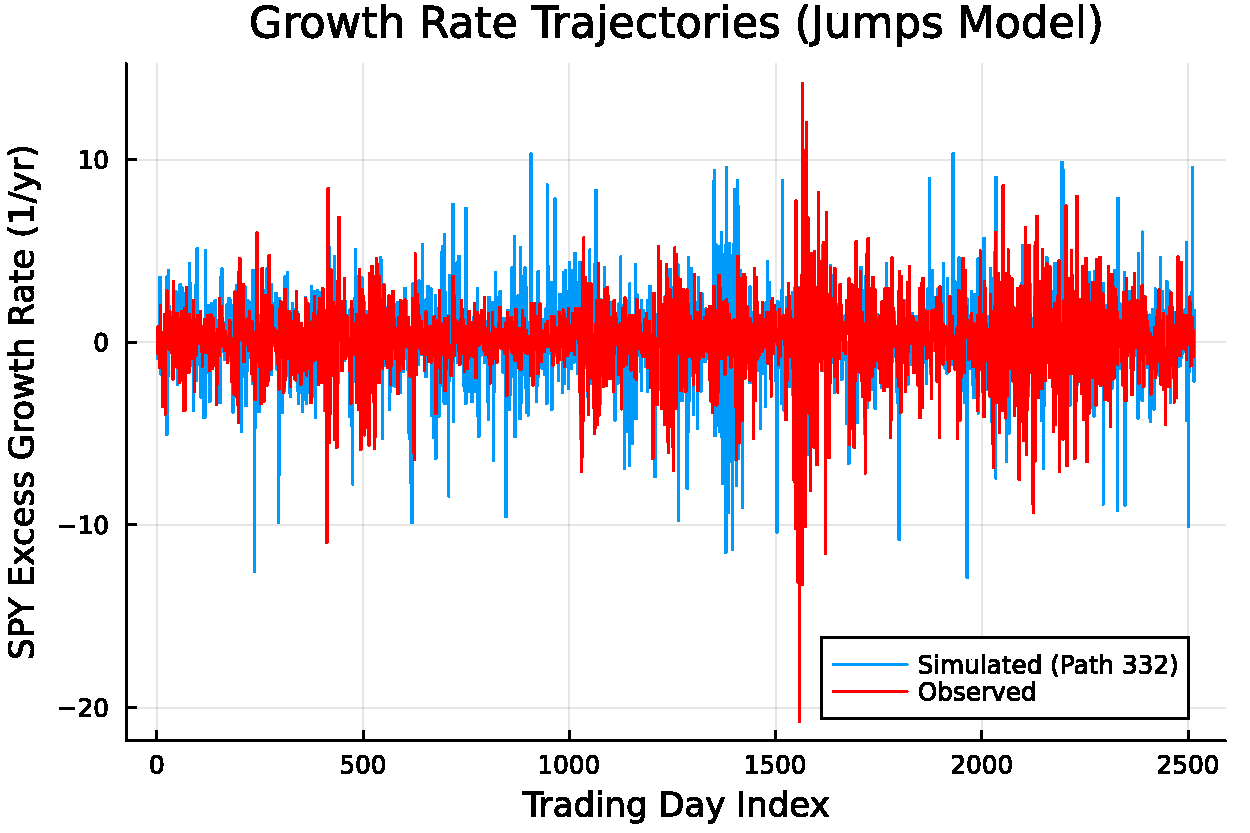
\includegraphics[width=\textwidth]{Fig-SPY-90-InSample-Return-Trajectories-WJ.pdf}
        \caption{Growth rate trajectories}
    \end{subfigure}
    \vspace{0.3cm}
    \begin{subfigure}[b]{0.48\textwidth}
        \centering
        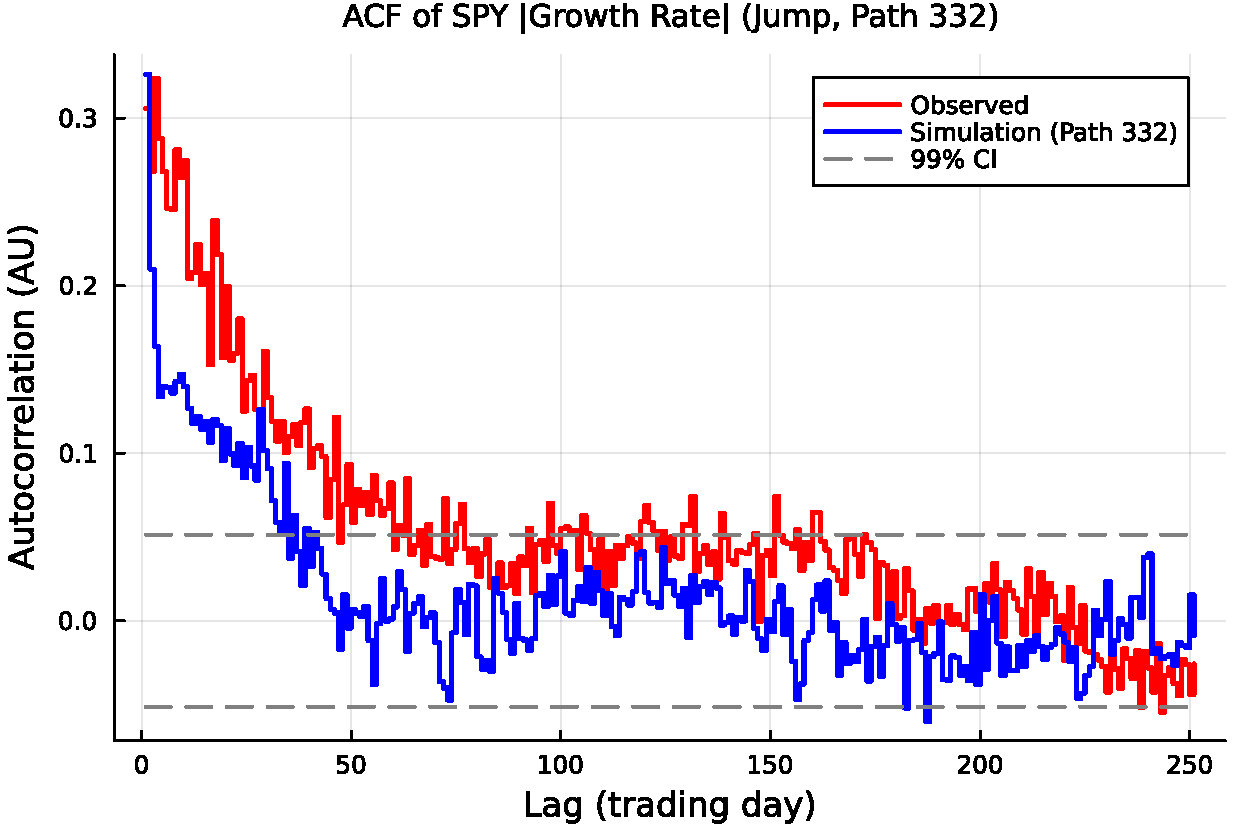
\includegraphics[width=\textwidth]{Fig-SPY-90-ACF-Absolute-Growth-WJ.pdf}
        \caption{Absolute growth autocorrelation}
    \end{subfigure}
    \hfill
    \begin{subfigure}[b]{0.48\textwidth}
        \centering
        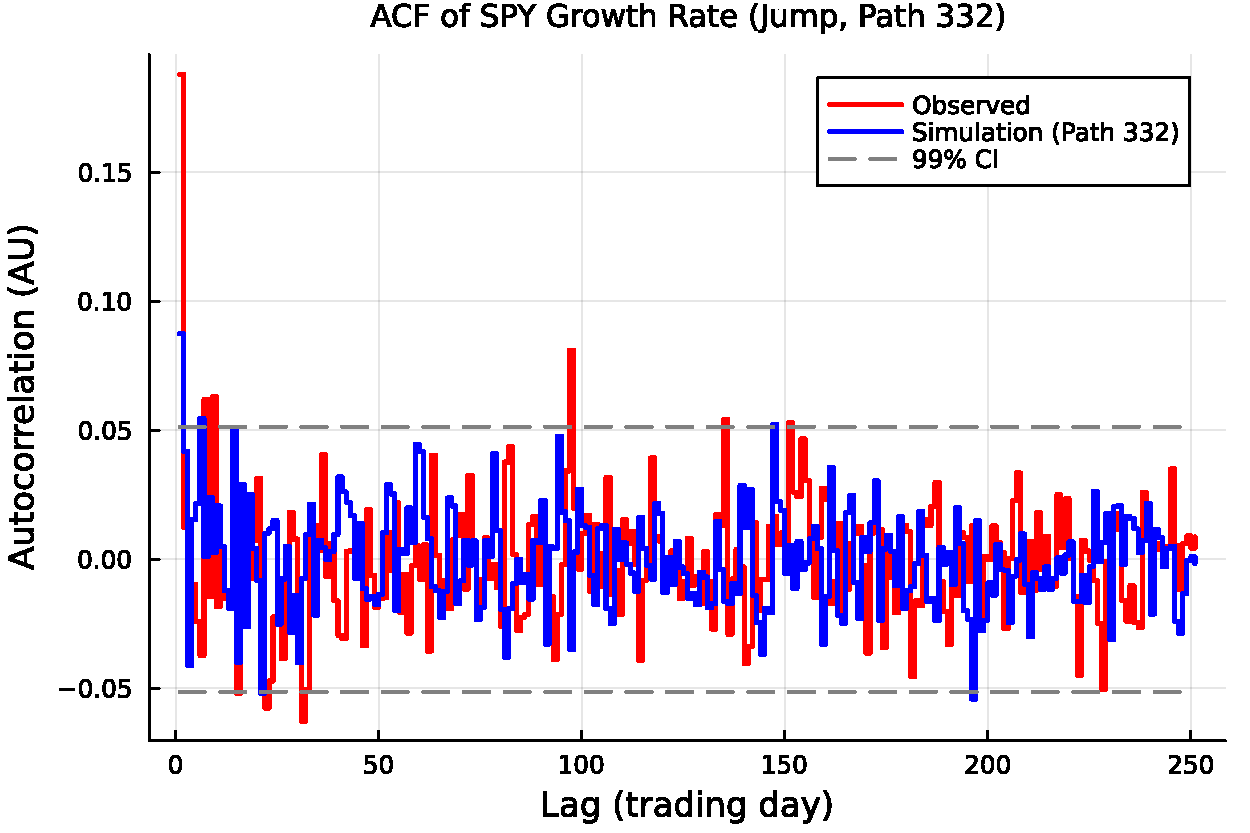
\includegraphics[width=\textwidth]{Fig-SPY-90-ACF-Growth-WJ.pdf}
        \caption{Growth autocorrelation function}
    \end{subfigure}
    \caption{Performance of the hybrid jumps model using $N=90$ states.}
    \label{fig:wj_90_combo}
\end{figure}
\FloatBarrier

\subsection{Out-of-sample performance}

Out-of-sample simulations remained statistically consistent, with KS and AD pass rates of 83.2 percent and 80.0 percent, respectively (Figure \ref{fig:wj_90_oos_combo}). This analysis utilized 277 trading days of unseen data from January 2, 2024, to February 7, 2025, and the results show the expected performance degradation relative to in-sample training while preserving realistic market behavior.

The correlation-distance distribution is centered at a mean distance of 1.0, indicating temporal independence between simulated paths and the historical trajectory (Figure \ref{fig:oos_correlation_distance}). The correlation distance, defined as $(1-\rho)$, measures the temporal alignment between simulated paths and the observed historical trajectory. This result is favorable in the context of quantitative finance because it confirms that the generative framework produces independent stochastic realizations that capture the stylized facts of the market without violating the efficient markets hypothesis by attempting to predict specific events \cite{fama_efficient_1970}. This underscores the distinction between a generative framework intended for stress testing and a forecasting tool intended for point prediction \cite{assefa_generating_2021, kwon_can_2024}.

Out-of-sample volatility differed by approximately 31.87 percent, yet volatility clustering persisted in subplot (c) (Figure \ref{fig:wj_90_oos_combo}). Unlike the standard Markov transition matrix, which decays rapidly, the Poisson jump mechanism successfully mimics the sticky nature of market volatility in unseen conditions. These results validate the hybrid framework as a robust tool for producing synthetic time series that remain statistically consistent with the underlying stochastic process \cite{cont_empirical_2001, ryden_stylized_1998, bulla_stylized_2006}.

\begin{figure}[htpb]
    \centering
    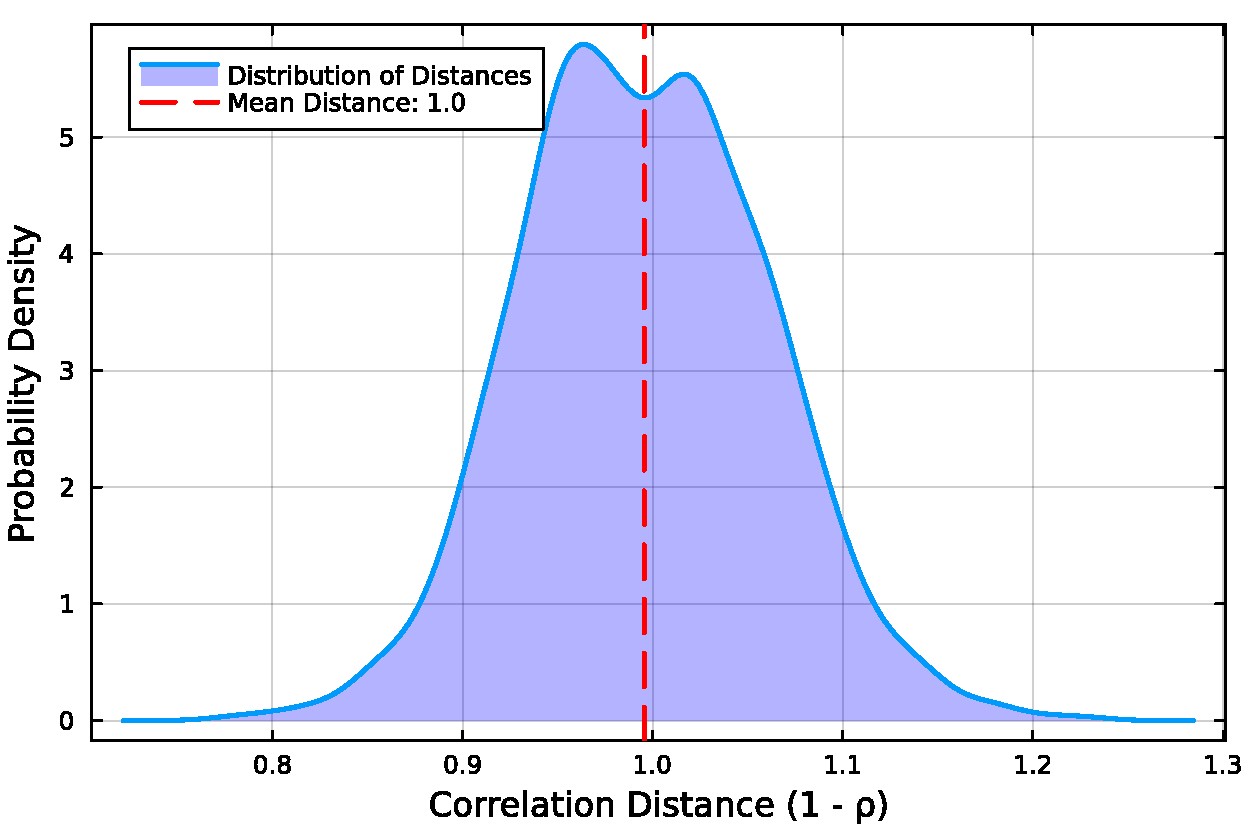
\includegraphics[width=0.7\textwidth]{Fig-SPY-90-OOS-CorrelationDistance-WJ.pdf}
    \caption{Distribution of correlation distances for 1,000 simulated paths. The mean distance of 1.0 for the correlation distance $(1-\rho)$ confirms the generation of independent realizations consistent with the efficient markets hypothesis.}
    \label{fig:oos_correlation_distance}
\end{figure}

\begin{figure}[htpb]
    \centering
    \begin{subfigure}[b]{0.48\textwidth}
        \centering
        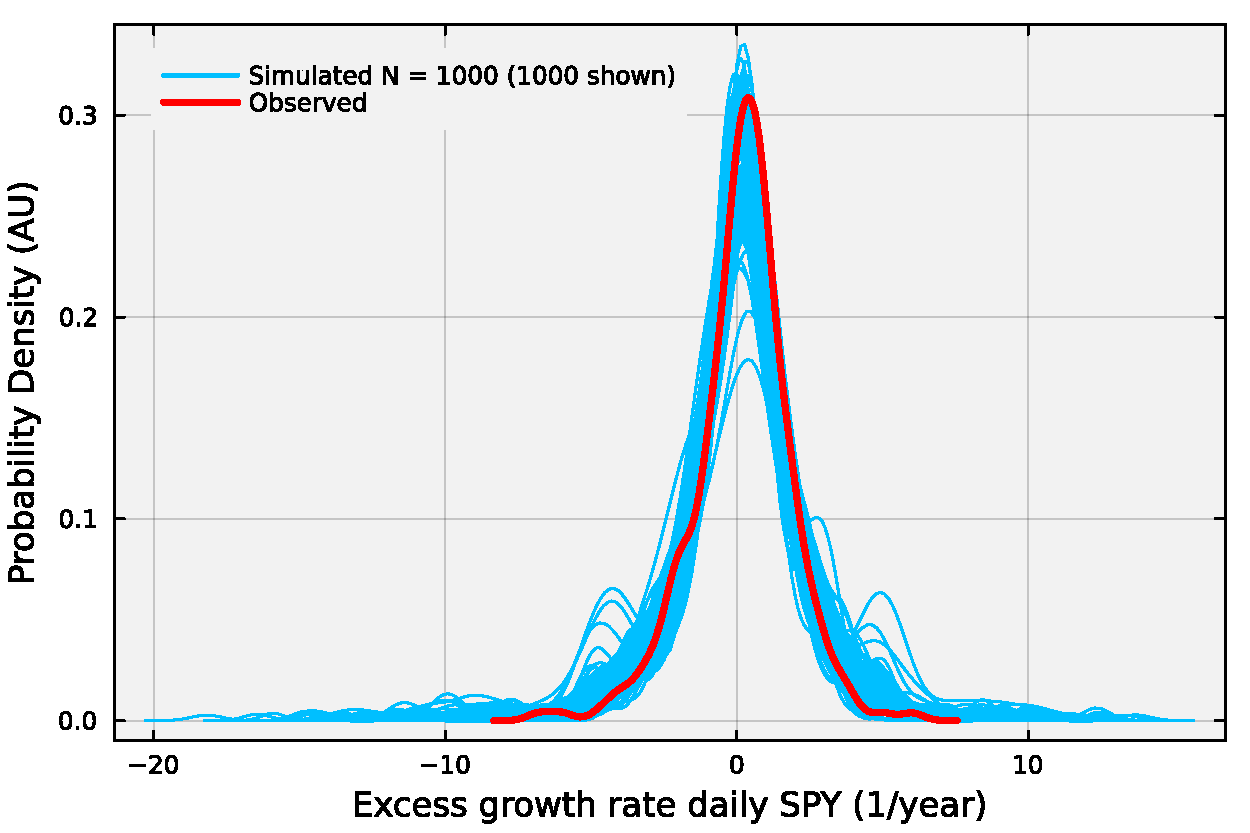
\includegraphics[width=\textwidth]{Fig-SPY-90-ExcessGrowthRate-Probability-Density-HMM-out-of-sample.pdf}
        \caption{Probability density comparison}
    \end{subfigure}
    \hfill
    \begin{subfigure}[b]{0.48\textwidth}
        \centering
        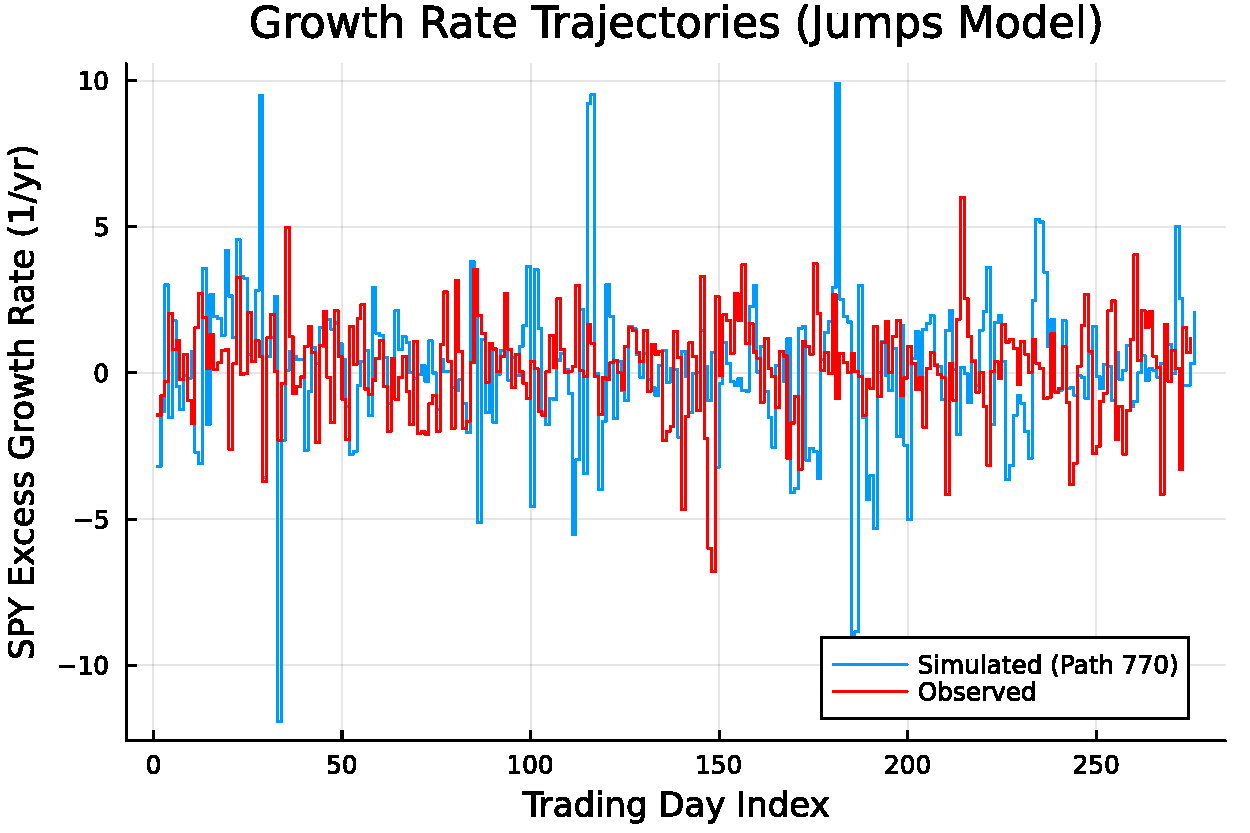
\includegraphics[width=\textwidth]{Fig-SPY-90-OOS-Return-Trajectories-WJ.pdf}
        \caption{Growth rate trajectories}
    \end{subfigure}
    \vspace{0.3cm}
    \begin{subfigure}[b]{0.48\textwidth}
        \centering
        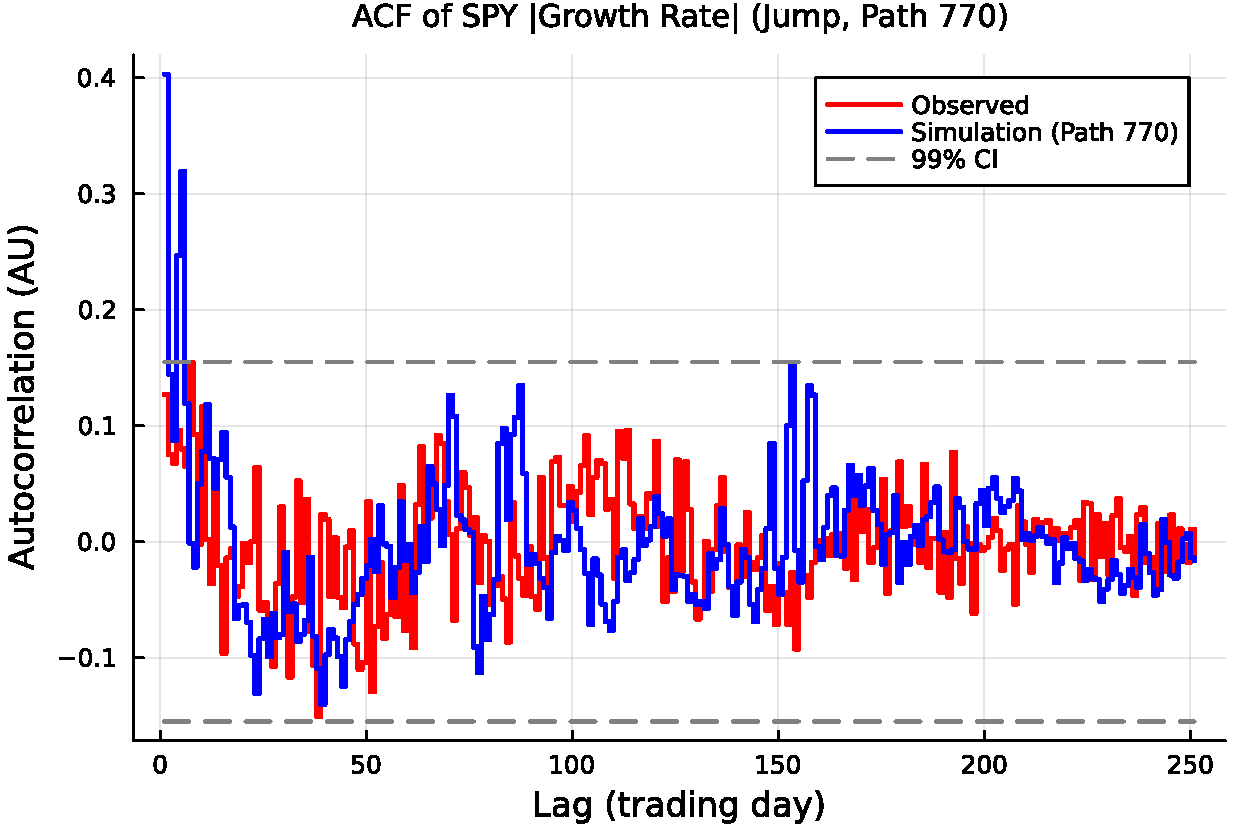
\includegraphics[width=\textwidth]{Fig-SPY-90-ACF-Absolute-Growth-WJ-OOS.pdf}
        \caption{Absolute growth autocorrelation}
    \end{subfigure}
    \hfill
    \begin{subfigure}[b]{0.48\textwidth}
        \centering
        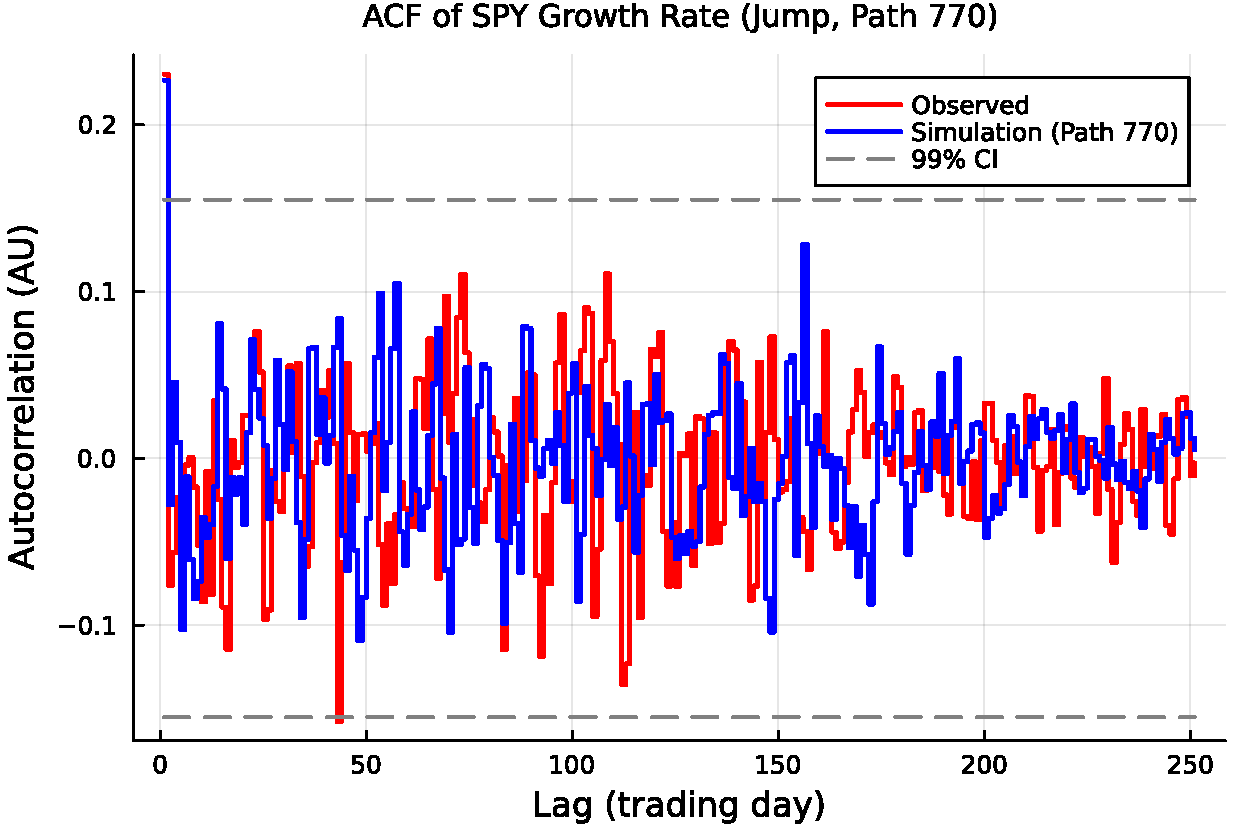
\includegraphics[width=\textwidth]{Fig-SPY-90-ACF-Growth-WJ-OOS.pdf}
        \caption{Growth autocorrelation function}
    \end{subfigure}
    \caption{Out-of-sample performance of the hybrid jumps model using $N=90$ states.}
    \label{fig:wj_90_oos_combo}
\end{figure}

\newpage
\section*{Conclusion}

This study introduced a hybrid hidden Markov modeling framework tailored for replicating the statistical regularities of empirical equity returns. By integrating a quantile-discretized state space with a Poisson-driven jump-duration mechanism, we developed a generative framework capable of capturing the leptokurtic distributions and volatility clustering characteristic of the SPY exchange-traded fund. Our results confirm that while increasing the state resolution to $N=90$ provides the necessary granularity to characterize the central mass of the return distribution, standard Markovian transitions alone are insufficient to reproduce higher-order temporal dependencies. The inclusion of discontinuous shocks through a jump-diffusion extension is essential to force the model into persistent extreme-volatility regimes, thereby replicating the ARCH effect identified in historical data.

Statistical validation using Kolmogorov-Smirnov and Anderson-Darling tests demonstrated exceptional in-sample consistency, with pass rates exceeding 98 percent. Although the out-of-sample performance showed a predictable decrease in fidelity, the hybrid model maintained a strong baseline with pass rates of 83.2 percent and 79.1 percent, respectively. Furthermore, the correlation distance analysis confirmed that our framework produces independent realizations that remain uncorrelated with specific historical timing; this satisfies the fundamental requirements of the efficient markets hypothesis and distinguishes our generative methodology from predictive forecasting tools \cite{fama_efficient_1970, assefa_generating_2021, kwon_can_2024}. The proposed framework offers a computationally efficient and empirically grounded alternative to standard likelihood-based estimation methods. By bypassing the complexities of the expectation-maximization algorithm through direct frequentist counting, the model remains well-suited for large-scale stress testing and risk management applications \cite{ohara_market_1998, manganelli_2004, glasserman_monte_2003}. Future research could extend this discrete-state logic to multi-asset portfolios or incorporate foundation models for inference to further refine the detection of Markov jump processes in higher-frequency data \cite{dias_mixture_2010, berghaus_foundation_2025}. Ultimately, the hybrid hidden Markov model serves as a capable foundation for simulating realistic market dynamics and generating synthetic time series that remain statistically consistent with underlying market regimes \cite{nguyen_hidden_2018, hamilton_regime_2018}.

\section*{Conflict of Interest Statement}
The authors declare that the research was conducted without any commercial or financial relationships that could potentially create a conflict of interest.

\section*{Author Contributions}
J.V. directed the study. A.A. developed the Julia model and simulation code, conducted the in-sample and out-of-sample analysis, and generated the figures. Both authors edited and reviewed the final manuscript.

\section*{Data Availability Statement}
The Julia model code and simulation scripts are available under an MIT software license from the GitHub repository: \url{https://github.com/altashly1/HMM-withJumps.git}

\newpage
\bibliographystyle{IEEEtran}
\bibliography{References}

\newpage
\appendix
\section{Algorithm implementation details}
\label{app:algo}

\begin{algorithm}[htpb]
\caption{Empirical hidden Markov model construction via Laplace partitioning}
\label{alg:build}
\begin{algorithmic}[1]
\REQUIRE Price history $P_{1:T}$, Risk-free rate $r_f$, Number of states $N$
\ENSURE Transition matrix $\mathbf{T}$, Parametric quantile boundaries $\mathcal{Q}$
\STATE Compute excess growth rates $R_t = \frac{1}{\Delta t} \ln(P_t / P_{t-1}) - r_f$ for all $t$.
\STATE Fit Laplace parameters $(\mu_L, b_L)$ to the series $\mathbf{R}$ using maximum-likelihood estimation.
\STATE Define state boundaries $q_k = F_L^{-1}(k/N; \mu_L, b_L)$ for $k \in \{1, \dots, N-1\}$, where $F_L^{-1}$ is the inverse cumulative distribution function of the Laplace distribution.
\STATE Assign each return $R_t$ to a discrete state $s_t \in \{1, \dots, N\}$ based on the boundaries in $\mathcal{Q}$.
\STATE Initialize count matrix $\mathbf{C} \in \mathbb{R}^{N \times N}$ and transition matrix $\mathbf{T} \in \mathbb{R}^{N \times N}$ with zeros.
\FOR{$t = 1$ to $T-1$}
    \STATE Identify transition $i = s_t$ to $j = s_{t+1}$.
\STATE $\mathbf{C}_{i,j} \leftarrow \mathbf{C}_{i,j} + 1$.
\ENDFOR
\FOR{$i = 1$ to $N$}
    \STATE $\mathbf{T}_{i,:} \leftarrow \mathbf{C}_{i,:} / \sum_{j=1}^{N} \mathbf{C}_{i,k}$ \COMMENT{Row-wise normalization}
\ENDFOR
\RETURN $\mathbf{T}, \mathcal{Q}$
\end{algorithmic}
\end{algorithm}

\begin{algorithm}[htpb]
\caption{Hybrid jump-diffusion simulation with persistent volatility}
\label{alg:sim}
\begin{algorithmic}[1]
\REQUIRE Model parameters $\mathbf{T}, \bar{\pi}, \epsilon, \lambda$, Total Steps $M$
\ENSURE Simulated state sequence $S_{1:M}$
\STATE Define tail-states $\mathcal{S}_{bottom} = \{1, 2, 3\}$ and $\mathcal{S}_{top} = \{N-2, N-1, N\}$.
\STATE Sample initial state $S_1 \sim \text{Categorical}(\bar{\pi})$.
\STATE Set $counter \leftarrow 2$.
\WHILE{$counter \le M$}
    \STATE Sample $u \sim \text{Uniform}(0, 1)$.
    \IF{$u < \epsilon$} 
        \STATE Sample jump-duration $K \sim \text{Poisson}(\lambda)$.
        \FOR{$j = 1$ to $K$ while $counter \le M$}
            \STATE Sample $w \sim \text{Uniform}(0, 1)$.
            \IF{$w < 0.52$} 
                \STATE $S_{counter} \sim \text{Uniform}(\mathcal{S}_{bottom})$ \COMMENT{Heuristic bias toward negative returns}
            \ELSE
                \STATE $S_{counter} \sim \text{Uniform}(\mathcal{S}_{top})$ 
            \ENDIF
            \STATE $counter \leftarrow counter + 1$.
        \ENDFOR
    \ELSE
        \STATE Sample $S_{counter} \sim \text{Categorical}(\mathbf{T}_{S_{counter-1}, :})$.
        \STATE $counter \leftarrow counter + 1$.
    \ENDIF
\ENDWHILE
\RETURN $S_{1:M}$
\end{algorithmic}
\end{algorithm}

\begin{algorithm}[htpb]
\caption{State decoding and continuous return reconstruction via MLE}
\label{alg:decode}
\begin{algorithmic}[1]
\REQUIRE Simulated state sequence $S_{1:M}$, Historical excess growth rates $\mathbf{R}$, Quantile boundaries $\mathcal{Q}$
\ENSURE Reconstructed continuous growth rates $\hat{R}_{1:M}$
\STATE Initialize an empty dictionary $\mathcal{D}$ to store state-specific data.
\FOR{$k = 1$ to $N$}
    \STATE Identify the historical returns falling within the $k$-th quantile bin: $\mathcal{D}_k = \{R_t \mid Q_{k-1} < R_t \le Q_k\}$.
\STATE Estimate the local mean $\mu_k = \frac{1}{|\mathcal{D}_k|} \sum_{R \in \mathcal{D}_k} R$.
\STATE Estimate the local standard deviation $\sigma_k = \sqrt{\frac{1}{|\mathcal{D}_k|} \sum_{R \in \mathcal{D}_k} (R - \mu_k)^2}$.
\ENDFOR
\STATE Initialize the reconstructed return vector $\mathbf{\hat{R}}$ of length $M$.
\FOR{$t = 1$ to $M$}
    \STATE Retrieve the simulated state $k = S_t$.
\STATE Sample the continuous growth rate $\hat{R}_t$ from the normal distribution $\mathcal{N}(\mu_k, \sigma_k)$.
\ENDFOR
\RETURN $\hat{R}_{1:M}$
\end{algorithmic}
\end{algorithm}

\section{Sensitivity analysis: low-resolution models}
\label{app:sensitivity}

This section provides the results for lower state resolutions ($N=30$ and $N=60$) to demonstrate how state granularity impacts the model's ability to capture stylized facts. Table \ref{tab:sensitivity_results} summarizes the pass rates for the Kolmogorov-Smirnov and Anderson-Darling tests across these four cases. As the number of states decreases, the model maintains a high global distribution fit, though the precision in the extreme tail-regions slightly diminishes compared to the 90 state configuration.

\begin{table}[htpb]
\centering
\caption{Statistical consistency of simulated growth rates for lower state resolutions ($N=30$ and $N=60$) using a $p$-value cutoff of 0.05.}
\label{tab:sensitivity_results}
\begin{tabular}{@{}lccc@{}}
\toprule
\textbf{model type} & \textbf{number of states ($N$)} & \textbf{KS test pass rate} & \textbf{AD test pass rate} \\ \midrule
standard (no-jumps) & 60 & 99.4\% & 98.3\% \\
standard (no-jumps) & 30 & 99.2\% & 98.2\% \\ \midrule
hybrid (with jumps) & 60 & 99.3\% & 97.6\% \\
hybrid (with jumps) & 30 & 98.7\% & 97.7\% \\ \bottomrule
\end{tabular}
\end{table}

The following figures illustrate the performance of these low-resolution configurations. Figure \ref{fig:nj_30_appendix} and Figure \ref{fig:wj_30_appendix} show the results for 30 states, while Figure \ref{fig:nj_60_appendix} and Figure \ref{fig:wj_60_appendix} provide the comparison for 60 states.

\begin{figure}[htpb]
    \centering
    \begin{subfigure}[b]{0.48\textwidth}
        \centering
        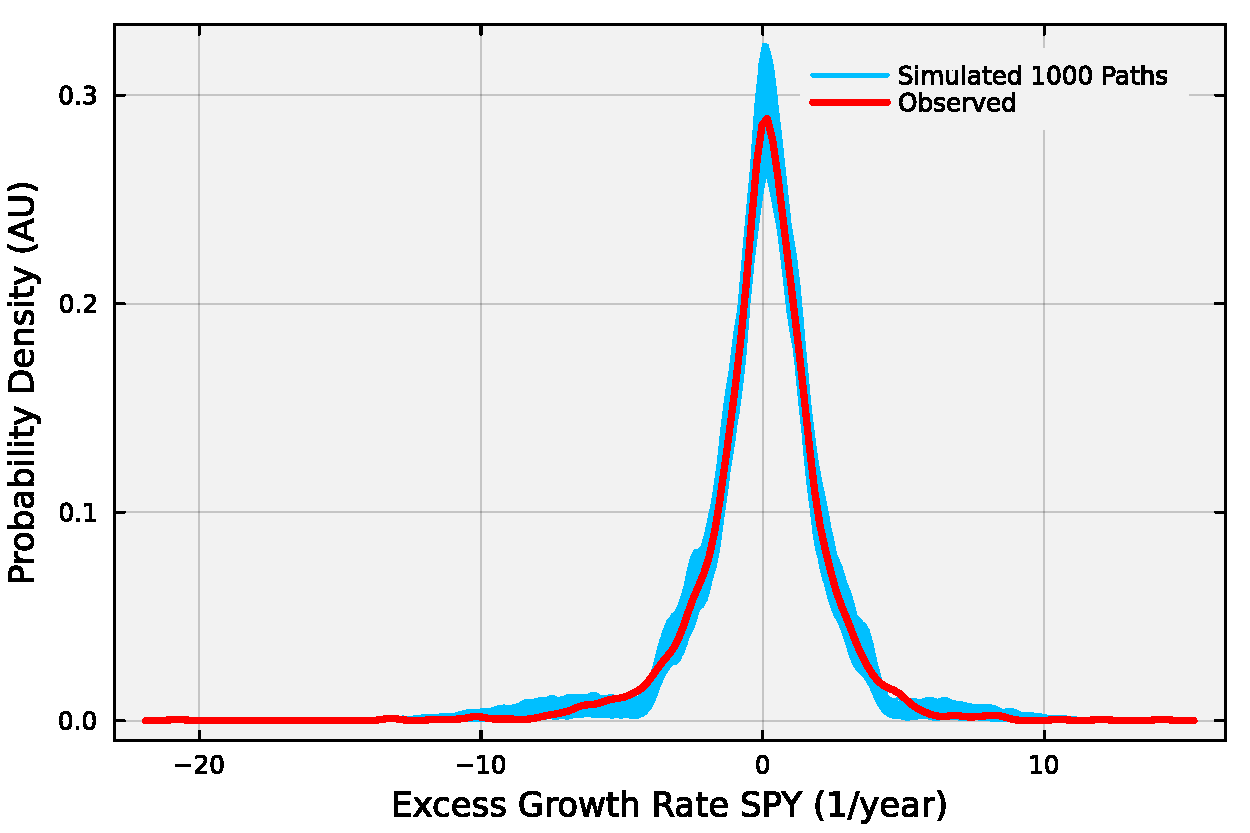
\includegraphics[width=\textwidth]{Fig-SPY-30-InSample-Density-Comparison-NJ.pdf}
        \caption{Density (standard)}
    \end{subfigure}
    \hfill
    \begin{subfigure}[b]{0.48\textwidth}
        \centering
        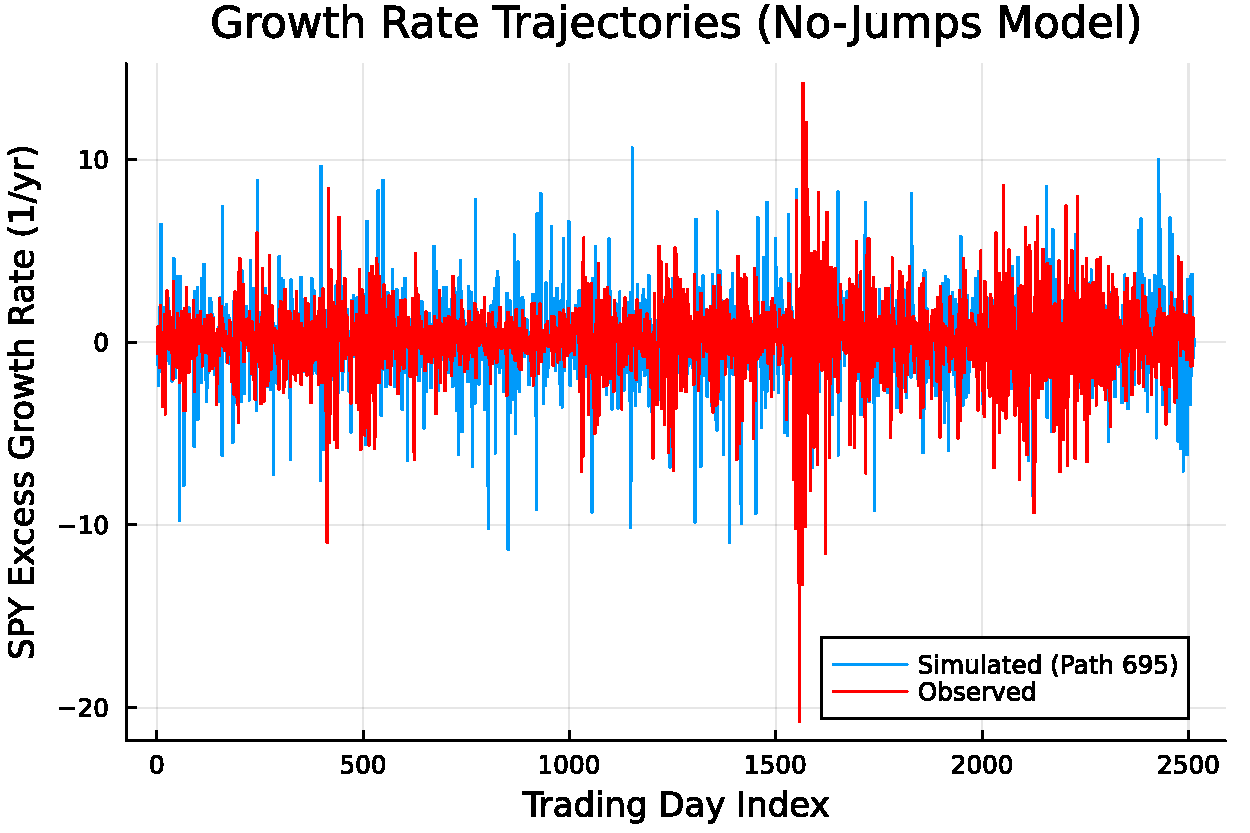
\includegraphics[width=\textwidth]{Fig-SPY-30-InSample-Return-Trajectories-NJ.pdf}
        \caption{Trajectories (standard)}
    \end{subfigure}
    \caption{Performance of the standard no-jumps model using $N=30$ states.}
    \label{fig:nj_30_appendix}
\end{figure}

\begin{figure}[htpb]
    \centering
    \begin{subfigure}[b]{0.48\textwidth}
        \centering
        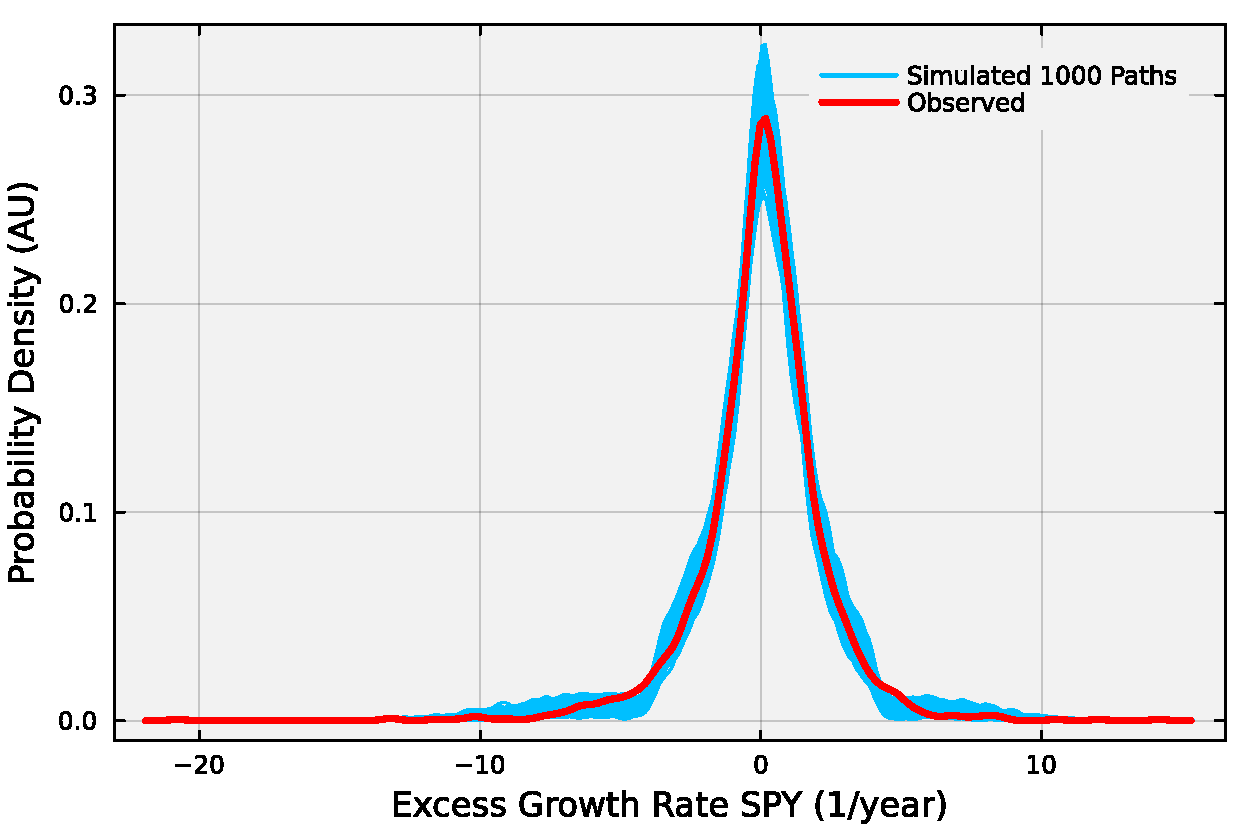
\includegraphics[width=\textwidth]{Fig-SPY-30-InSample-Density-Comparison-HMM-WJ.pdf}
        \caption{Density (hybrid)}
    \end{subfigure}
    \hfill
    \begin{subfigure}[b]{0.48\textwidth}
        \centering
        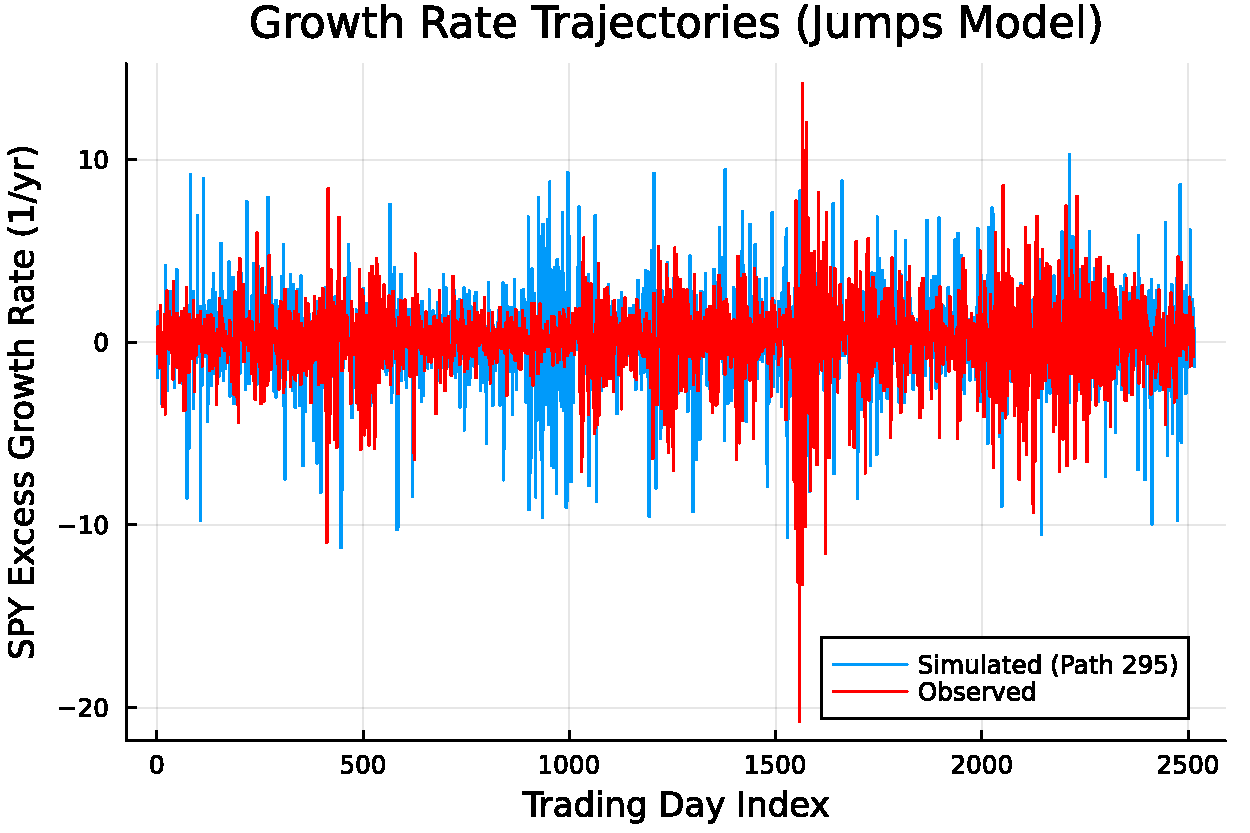
\includegraphics[width=\textwidth]{Fig-SPY-30-InSample-Return-Trajectories-WJ.pdf}
        \caption{Trajectories (hybrid)}
    \end{subfigure}
    \caption{Performance of the hybrid jumps model using $N=30$ states.}
    \label{fig:wj_30_appendix}
\end{figure}

\begin{figure}[htpb]
    \centering
    \begin{subfigure}[b]{0.48\textwidth}
        \centering
        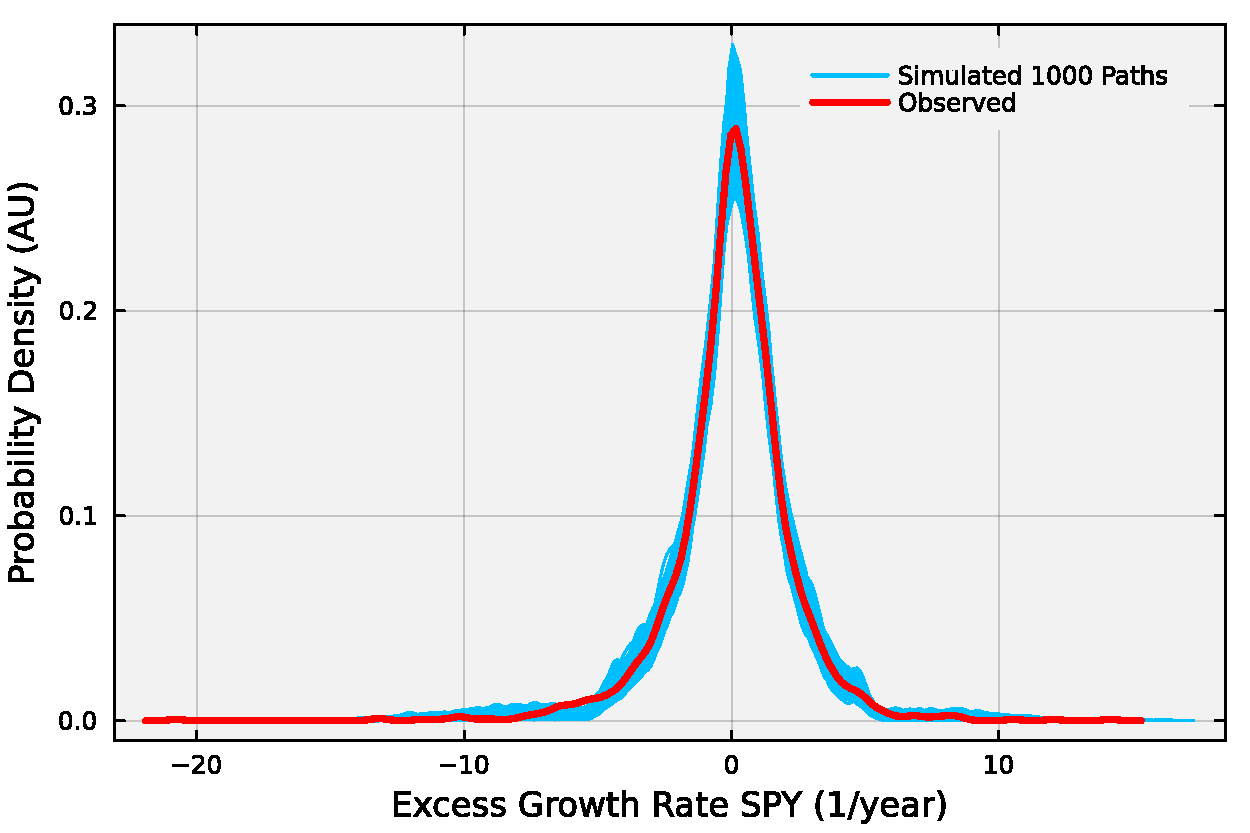
\includegraphics[width=\textwidth]{Fig-SPY-60-InSample-Density-Comparison-NJ.pdf}
        \caption{Density (standard)}
    \end{subfigure}
    \hfill
    \begin{subfigure}[b]{0.48\textwidth}
        \centering
        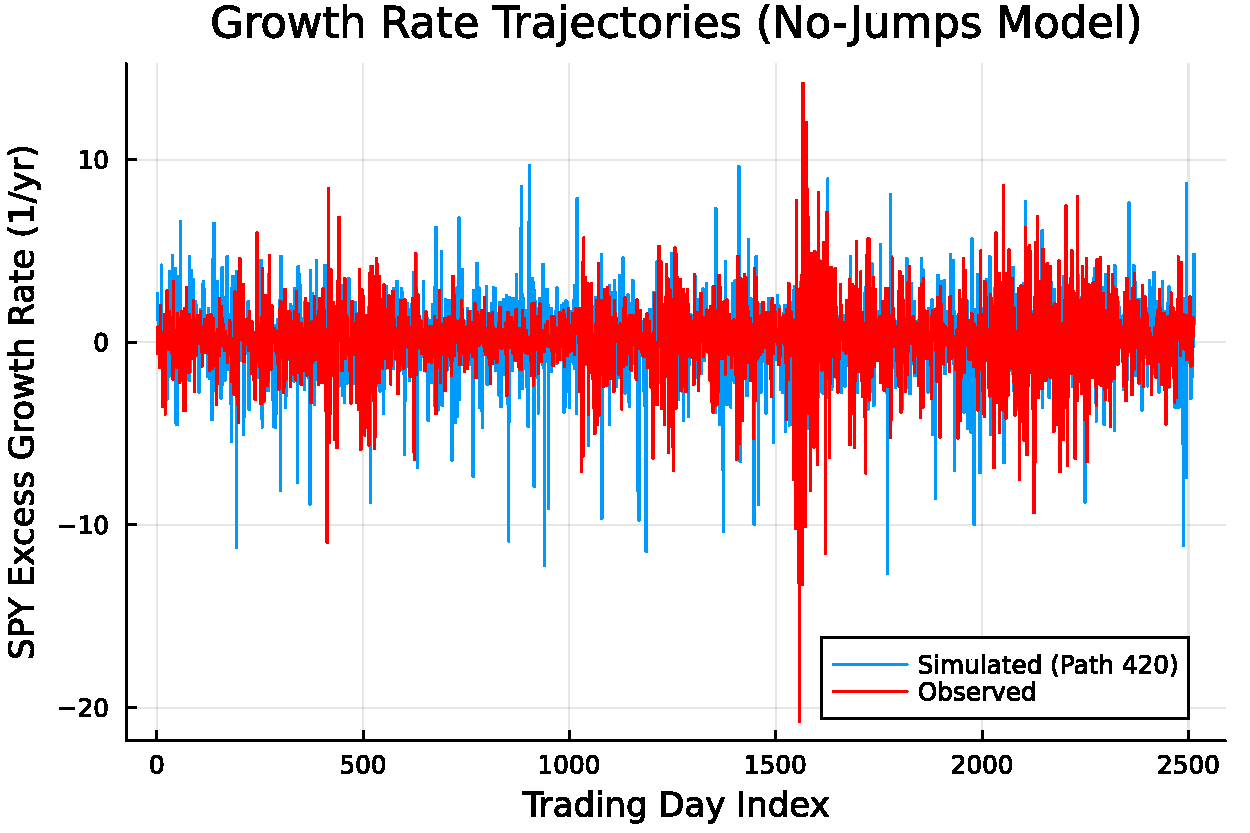
\includegraphics[width=\textwidth]{Fig-SPY-60-InSample-Return-Trajectories-NJ.pdf}
        \caption{Trajectories (standard)}
    \end{subfigure}
    \caption{Performance of the standard no-jumps model using $N=60$ states.}
    \label{fig:nj_60_appendix}
\end{figure}

\begin{figure}[htpb]
    \centering
    \begin{subfigure}[b]{0.48\textwidth}
        \centering
        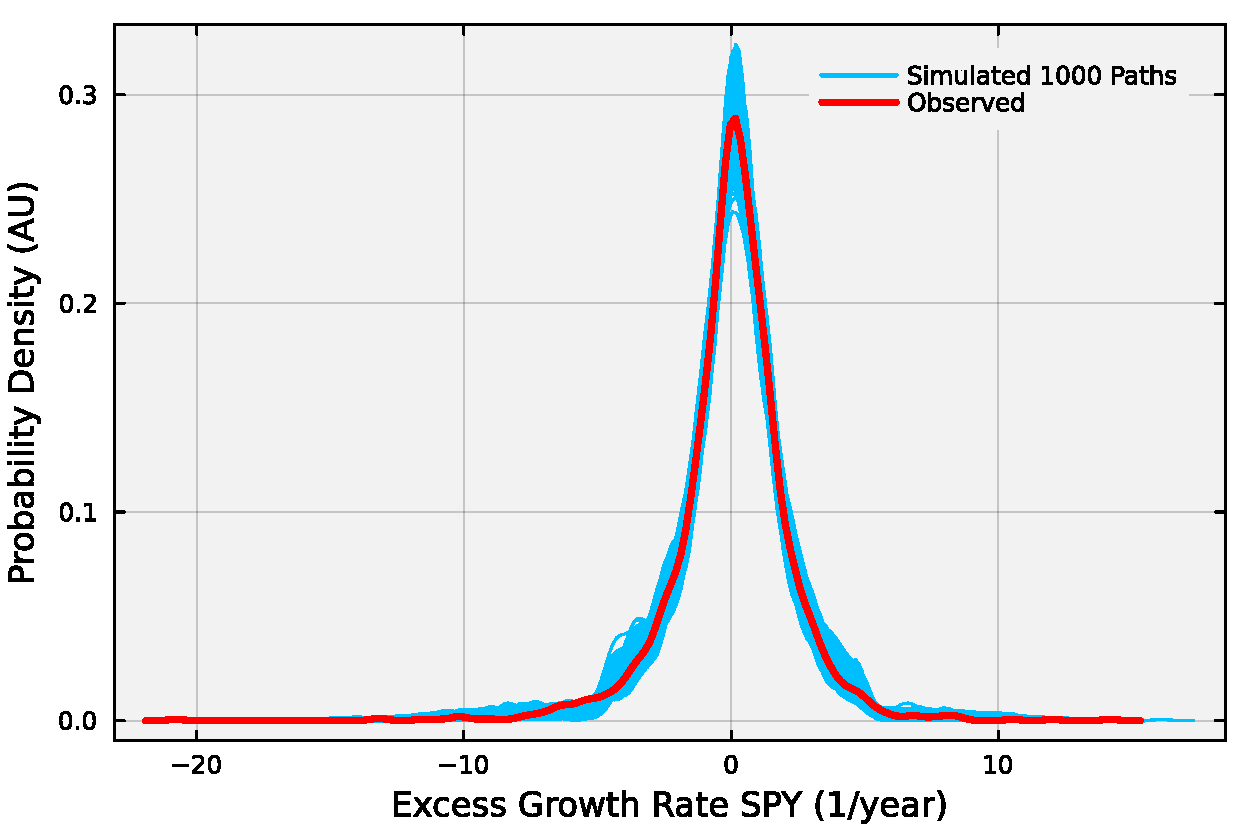
\includegraphics[width=\textwidth]{Fig-SPY-60-InSample-Density-Comparison-HMM-WJ.pdf}
        \caption{Density (hybrid)}
    \end{subfigure}
    \hfill
    \begin{subfigure}[b]{0.48\textwidth}
        \centering
        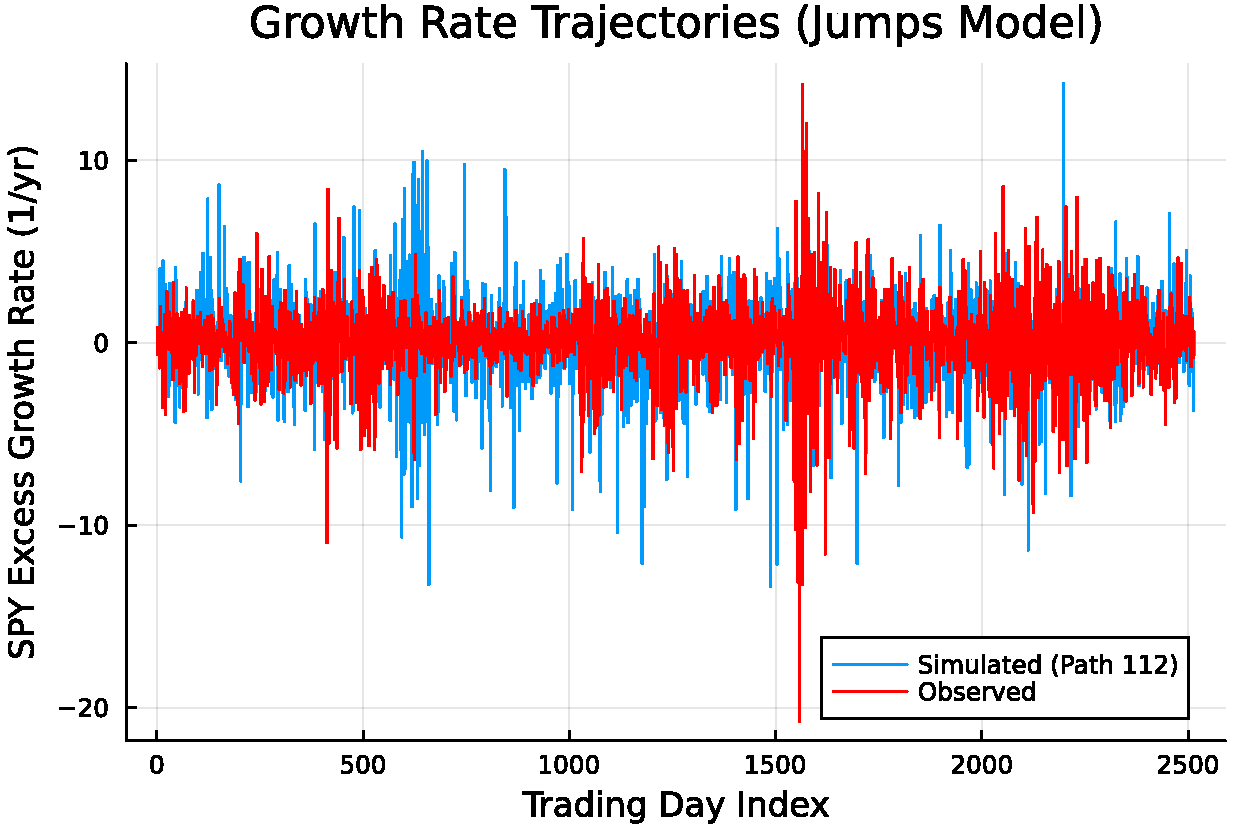
\includegraphics[width=\textwidth]{Fig-SPY-60-InSample-Return-Trajectories-WJ.pdf}
        \caption{Trajectories (hybrid)}
    \end{subfigure}
    \caption{Performance of the hybrid jumps model using $N=60$ states.}
    \label{fig:wj_60_appendix}
\end{figure}

\end{document}
